\section{Service Oriented Architecture}
\dbc{Use a more meaningful title that reflect the solution. Also, why are we talking about an initial phase? You can mention that we iterate through several designs. But it's not important to discuss each design in detail unless once design is essential to understand the other design. Ideally, present only the finalized design while adding a single para for each of the previous attempts.}

In the initial phase of WDIAS architecture, it proposed with a \acrfull{soa} as shown in the \ref{fi:proposed_soa}. Mainly it consist of 4 modules, namely:
- Import modules
Import modules are using for integration of data from different source which come in different data formats.
- Export modules
Export modules are using for data dissemination with different format which may required for different type of operations.
- Extension modules
Extension modules are capable of providing the data assimilation functionalities by providing some of key functionalities such as transformation, interpolation and validation. While data assimilation, existing timeseries may be modified or create new timeseries based on the system configurations.
- Adapter module
Adapter module is handling the complexity of integrating different data formats and storing them in the way that easy to search and retrieve.

\begin{figure}[htp]
    \centering
    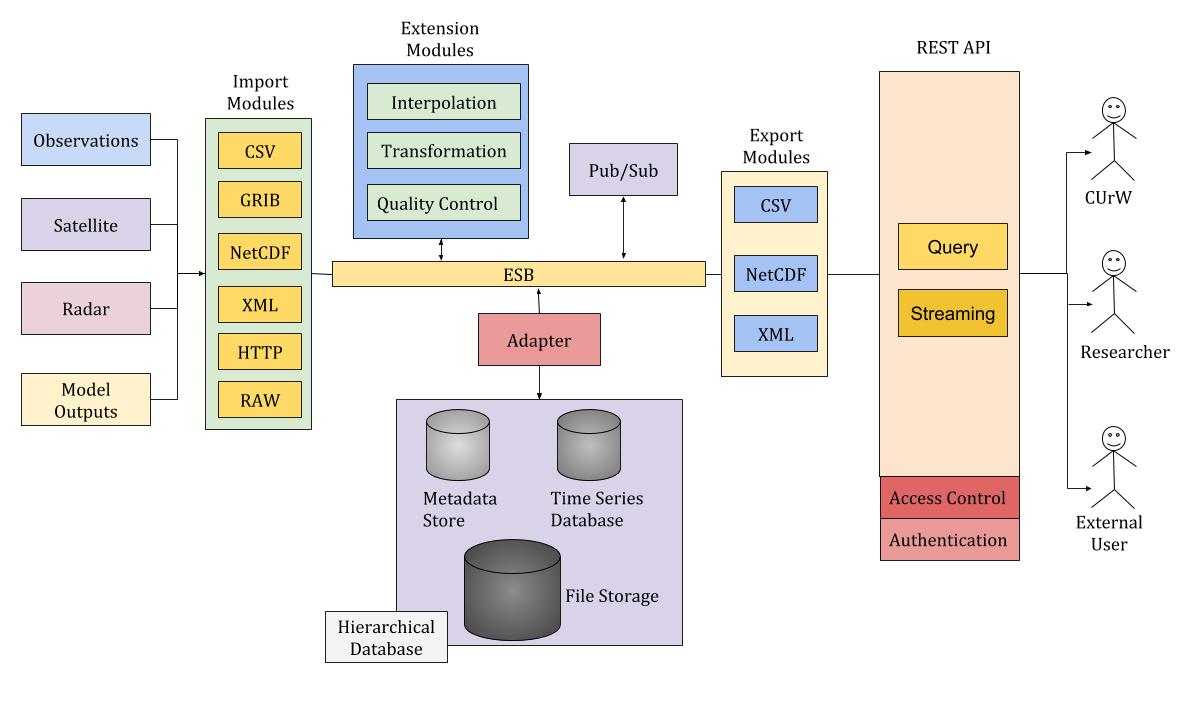
\includegraphics[width=1\textwidth]{soa/soa_v1.jpg}
    \caption{Service oriented architecture of \acrshort{wdias}.}
    \label{fi:proposed_soa}
\end{figure}

- \acrfull{esb}
While implementing a \acrfull{soa}, the \acrfull{esb} can provide capability to integrate different modules, since it is acting as a common layer for all of modules.
By default, \acrshort{esb} provides pub sub capabilities.
\acrshort{esb} mediator can be used to integrate the import, export and extension modules. \acrshort{esb} also support different transportation protocols such as HTTP and Web-Socket etc.

But \acrshort{esb} is not a better solution for data streaming or bulk data processing. Also \acrshort{esb} suffer from single point of failure, since all the messages are going though a common bus.

\section{Actor Model}

In the second phase of \acrshort{wdias}, the proposed architecture changed to use with Actor model after consider into the disadvantage of using \acrshort{esb}.

Brief about using actor model:
https://doc.akka.io/docs/akka/2.5.5/scala/guide/actors-motivation.html
\dbc{Give the URL as a reference.}

The typical SOA model, for example, usually has more dependent ESBs, with microservices using faster messaging mechanisms.  SOA also focuses on imperative programming, whereas microservices architecture focuses on a responsive-actor programming style.  Moreover, SOA models tend to have an outsized relational database, while microservices frequently use NoSQL or micro-SQL databases (which can be connected to conventional databases).  But the real difference has to do with the architecture methods used to arrive at an integrated set of services in the first place. (Refer:https://smartbear.com/learn/api-design/what-are-microservices/ )

- Add diagrams for handle on demand
- Add diagram for handle Async


AKKA vs ESB
ESB support to implement SOA. But SOA has limitations such as single point of failure, slower communication (can’t use for transfer data) etc. So, the microservice architecture get evolved and demanding for the moment. It has following benefits,
Follow the Single Responsibility Principle
Resilient/Flexible – failure in one service does not impact other services. If you have monolithic or bulky service errors in one service/module it can impact other modules/functionality.
High scalability – demanding services can be deployed in multiple servers to enhance performance and keep away from other services so that they don’t impact other services. Will be difficult to achieve the same with single, large monolithic service.
Easy to enhance – less dependency and easy to change and test
Low impact on other services – being an independent service, this has less chance to impact other services
Easy to understand since they represent the small piece of functionality
Ease of deployment
Freedom to choose technology – allows you to choose technology that is best suited for a particular functionality
